
\documentclass[12pt, a4paper]{article}
\usepackage{hyperref}
\hypersetup{
  colorlinks=true,
  linkcolor=blue,
  urlcolor=cyan,
}
\urlstyle{same}
\usepackage[utf8]{inputenc}
\usepackage{amsmath}
\usepackage{amsfonts}
\usepackage{amssymb}
\usepackage{graphicx}


\newtheorem{theorem}{Teorema.}
\newtheorem{lemma}[theorem]{Lema.}
\newtheorem{corollary}[theorem]{Corolario.}
\newtheorem{definition}[theorem]{Definici\'on:}
\newtheorem{example}[theorem]{Ejemplo:}
\newtheorem{problema}[theorem]{Problema:}
\newtheorem{remark}[theorem]{Observaci\'on:}

\usepackage{graphicx}
\usepackage[spanish]{babel}
%\usetheme{default}

\newcommand{\pp}{\mathbb{P}}
\newcommand{\zz}{\mathbb{Z}}
\newcommand{\rr}{\mathbb{R}}
\newcommand{\qq}{\mathbb{Q}}

\usepackage{tikz, tikz-3dplot}

\definecolor{cof}{RGB}{219,144,71}
\definecolor{pur}{RGB}{186,146,162}
\definecolor{greeo}{RGB}{91,173,69}
\definecolor{greet}{RGB}{52,111,72}

\date{}

\begin{document}
\title{Pr\'actico 1 ALGABO: Grafos y BFS.}
\author{Mauricio Velasco}
\maketitle{}
\begin{enumerate} 
\item Implemente una clase \texttt{Grafo} que represente un grafo dirigido \texttt{G} como lista de adyacencia. La clase debe recibe sólo el número de vértices del grafo e implementar las operaciones \verb G.nueva_arista(i,j) , \verb G.nuevo_vertice() y \verb G.print().
\begin{enumerate}
\item Escriba el c\'odigo de su implementaci\'on.
\item Cu\'anta memoria (como funci\'on de $n$) requiere su clase para representar:
\begin{enumerate}
\item Un grafo completo $K_n$.
\item Un grafo bipartito completo $K_{n,n}$
\item Un ciclo de longitud $n$.
\item Un \'arbol con $n$ v\'ertices.
\end{enumerate} 

\end{enumerate}

\item Visitamos todos los v\'ertices del grafo no dirigido con $V=\{1,\dots, 7\}$ y con aristas $E$ determinadas por $(1,2), (1,3)$ $(3,7), (3,6), (2,4)$ y $(2,5)$ iniciando en el v\'ertice $(2)$.
\begin{enumerate}
\item Escriba la lista de v\'ertices en el orden en el que los visitar\'iamos en BFS.
\item Hay otro orden posible adicional al que escribi\'o en el numeral anterior?
\item Cu\'antos \'ordenes posibles hay? Escr\'ibalos todos.
\item Generalizado el ejemplo anterior, cu\'antos \'ordenes BFS cree que hay para recorrer un \'arbol binario con $\ell$ niveles?.
\end{enumerate}

\item Sea $A$ la matriz de adyacencia de un grafo $G$. Demuestre que para cualquier entero positivo $k$ y para cualquier par de v\'ertices $i,j$ se tiene que $(A^{k})_{ij}$ es igual al n\'umero de caminos desde $i$ hasta $j$ de longitud $k$.

\item{Recuerde que un \'arbol es, por definici\'on, un grafo conexo y sin ciclos. Demuestre las siguientes afirmaciones:
\begin{enumerate}
\item Si $G$ es un grafo con $n$ v\'ertices y $m$ aristas entonces $m=O(n^2)$.
\item Todo \'arbol con $n$ v\'ertices tiene $n-1$ aristas.
\item Concluya que si $G$ es un grafo conexo con $m$ v\'ertices entonces $m=\Omega(n)$ y $m=O(n^2)$.
\end{enumerate}
}


\item Implemente una funci\'on que reciba un \texttt{Grafo} $H$ y el \'indice de un v\'ertice de $H$ y retorne un árbol breadth-first-search $T$ para $H$. El árbol $T$ debe ser una instancia de la clase \texttt{Grafo} del problema $(1)$.

\begin{enumerate}
\item Escriba el c\'odigo de su implementaci\'on.
\item Utilice su implementaci\'on en el grafo del siguiente dibujo iniciando en el v\'ertice $D$ 
\begin{center}
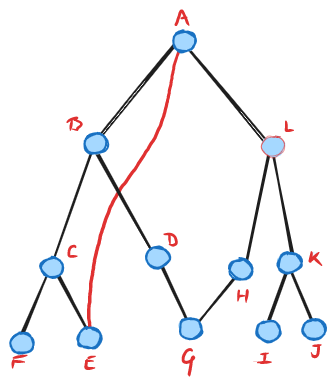
\includegraphics[scale=0.5]{grafo_1.png}
\end{center}
y dibuje el \'arbol $T$ obtenido.
\end{enumerate}


\end{enumerate}


\end{document}



